%%%%%%%%%%%%%%%%%%%%%%%%%%%%%%%%%%%%%%%%%%%%%%%%%%%%%%%%%%%%%%%%%%%%%%%%%%%%%

\chapter{La sonate op. 27}

\begin{figure}[!p]
  \begin{bigcenter}
    \begin{tabular}{lr}
      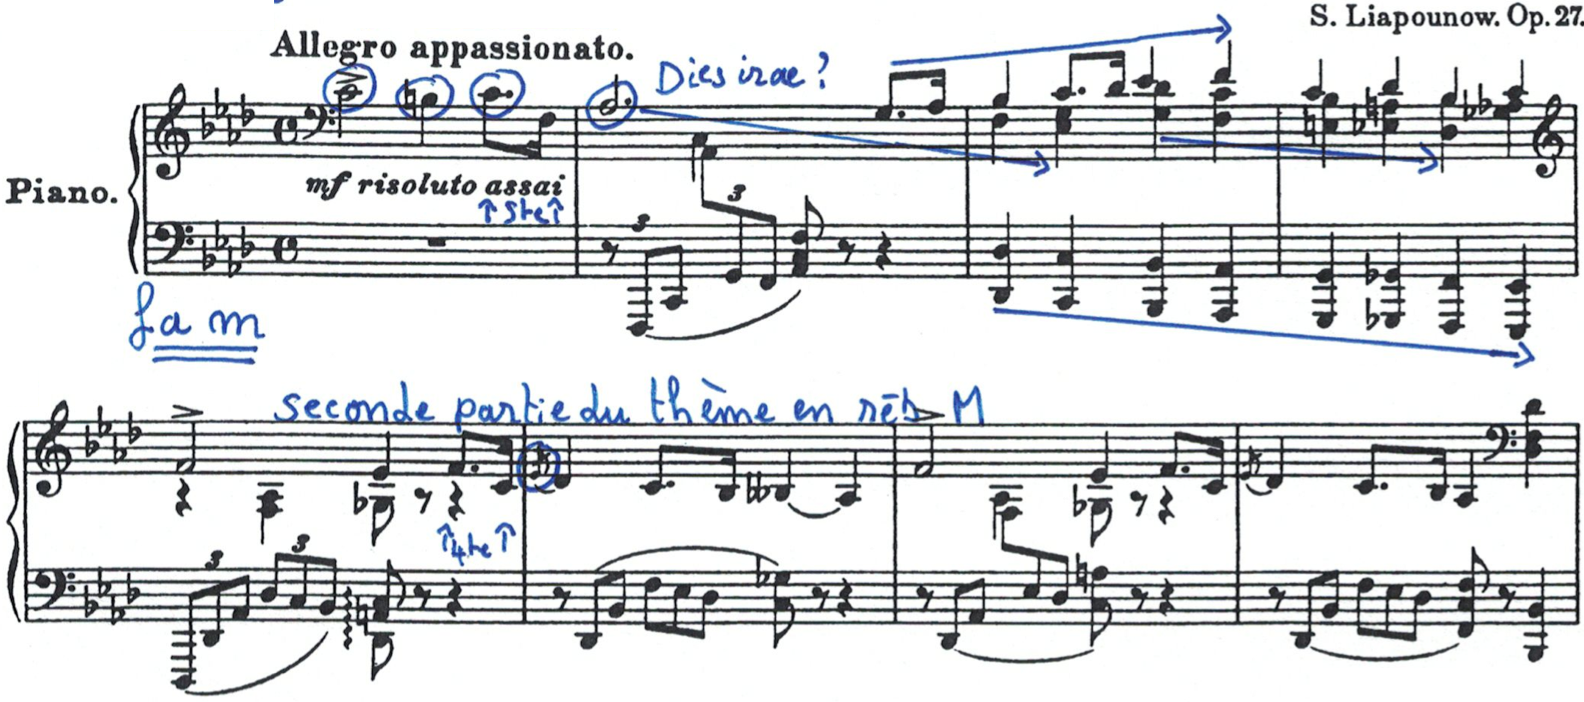
\includegraphics[width=12.5cm, keepaspectratio]{sonate-theme-A.png}
      &
      
\includegraphics[width=3cm, keepaspectratio]{op1-qr.png}
    \end{tabular}
  \end{bigcenter}
  \caption{\label{sonate-theme-1}Sonate en fa m Op.25, thème A.}
\end{figure}

\begin{figure}[!ht]
  \begin{bigcenter}
    \begin{tabular}{lr}
      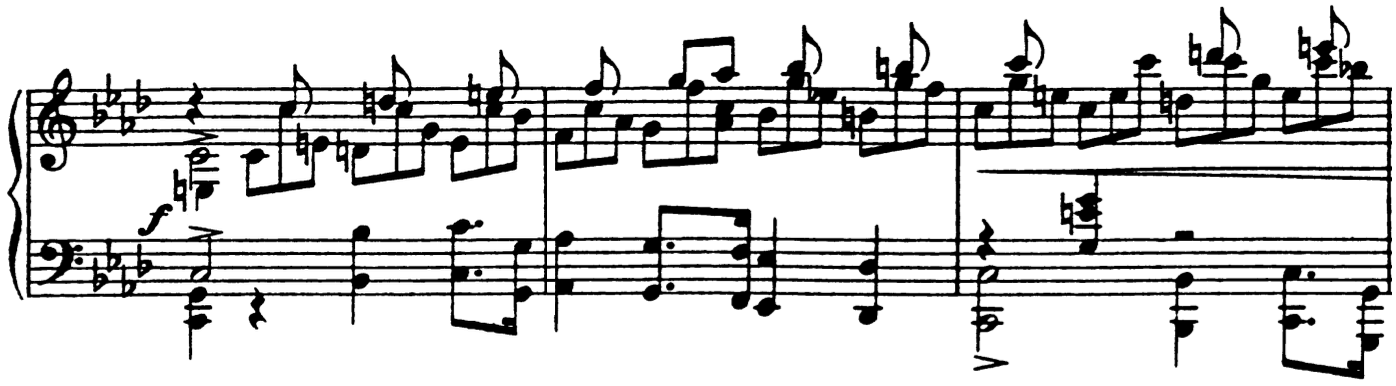
\includegraphics[width=12.5cm, keepaspectratio]{sonate-theme-A2.png}
      &
      
\includegraphics[width=3cm, keepaspectratio]{op1-qr.png}
    \end{tabular}
  \end{bigcenter}
  \caption{\label{sonate-theme-1}Sonate en fa m Op.25, thème A2.}
\end{figure}

\begin{figure}[!p]
  \begin{bigcenter}
    \begin{tabular}{lr}
      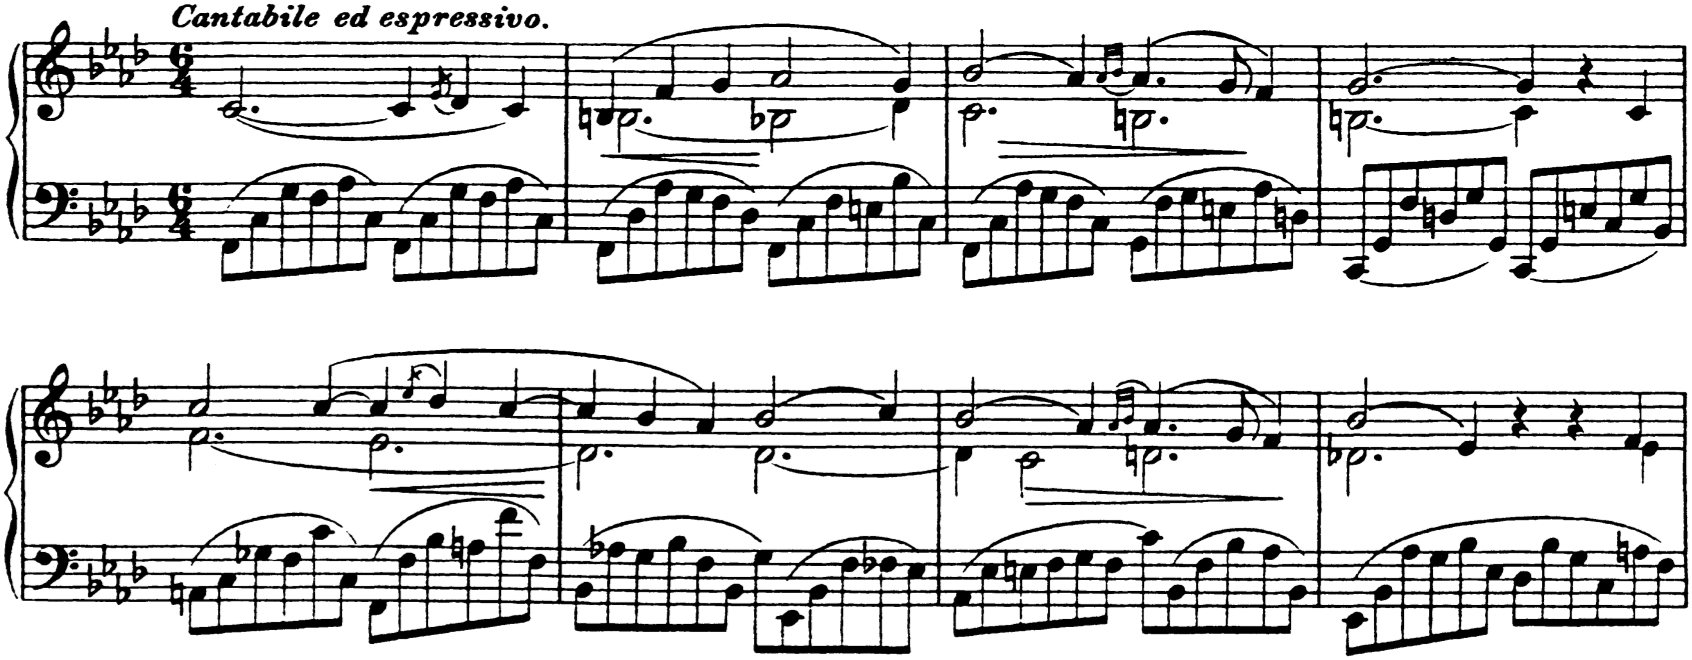
\includegraphics[width=12.5cm, keepaspectratio]{sonate-theme-B.png}
      &
      
\includegraphics[width=3cm, keepaspectratio]{op1-qr.png}
    \end{tabular}
  \end{bigcenter}
  \caption{\label{sonate-theme-1}Sonate en fa m Op.25, thème B.}
\end{figure}

\begin{figure}[!p]
  \begin{bigcenter}
    \begin{tabular}{lr}
      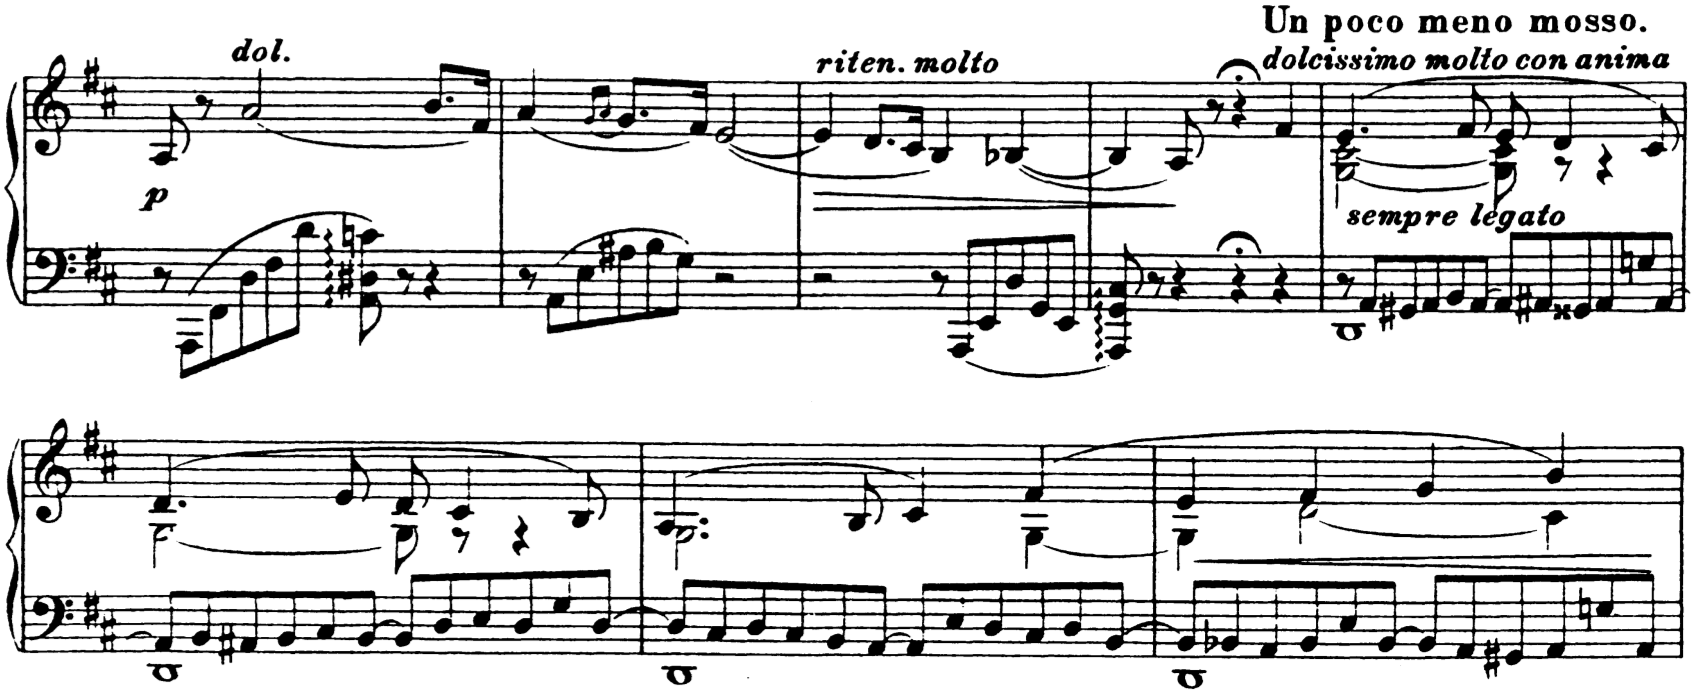
\includegraphics[width=12.5cm, keepaspectratio]{sonate-theme-C.png}
      &
      
\includegraphics[width=3cm, keepaspectratio]{op1-qr.png}
    \end{tabular}
  \end{bigcenter}
  \caption{\label{sonate-theme-1}Sonate en fa m Op.25, thème C.}
\end{figure}

\begin{figure}[!p]
  \begin{bigcenter}
    \begin{tabular}{lr}
      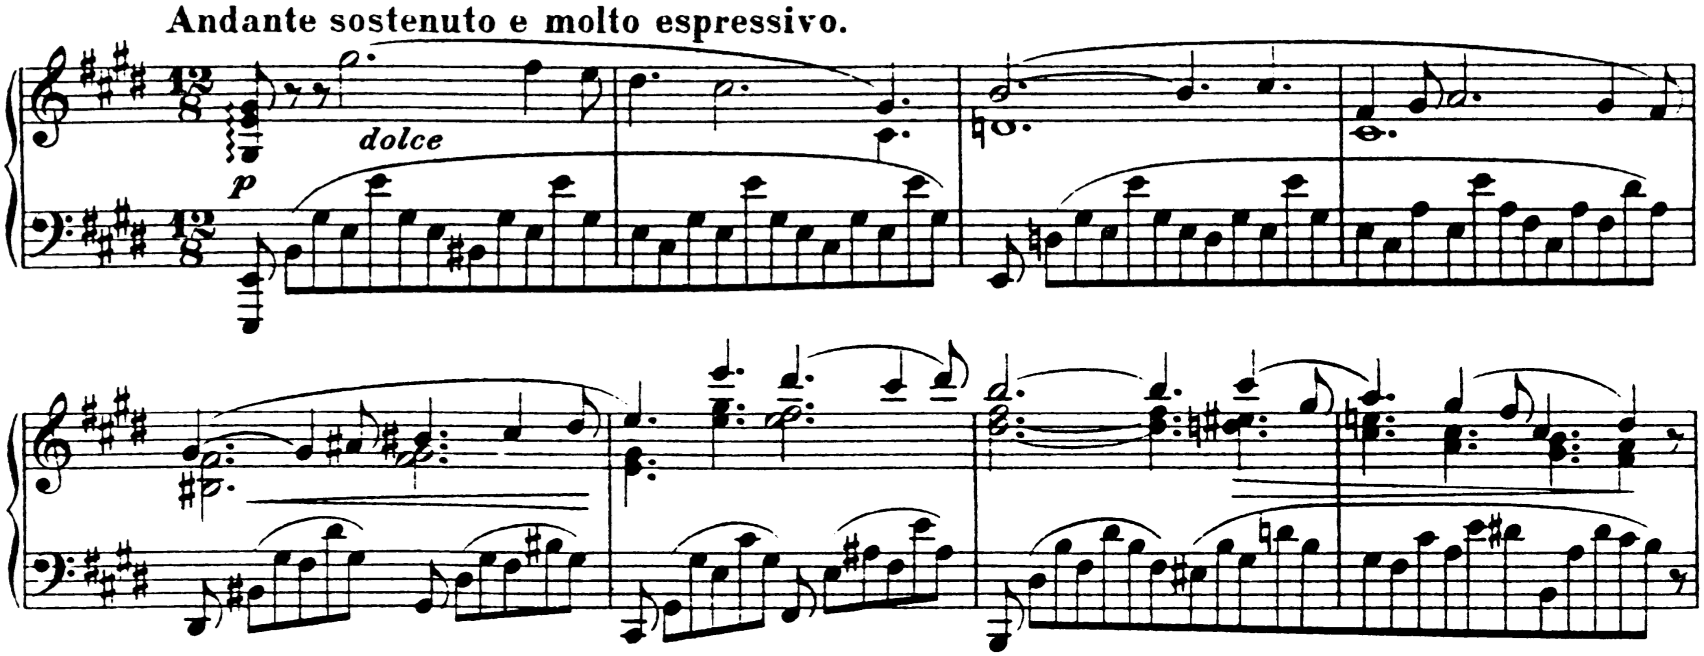
\includegraphics[width=12.5cm, keepaspectratio]{sonate-theme-D.png}
      &
      
\includegraphics[width=3cm, keepaspectratio]{op1-qr.png}
    \end{tabular}
  \end{bigcenter}
  \caption{\label{sonate-theme-1}Sonate en fa m Op.25, thème D.}
\end{figure}

\begin{figure}[!p]
  \begin{bigcenter}
    \begin{tabular}{lr}
      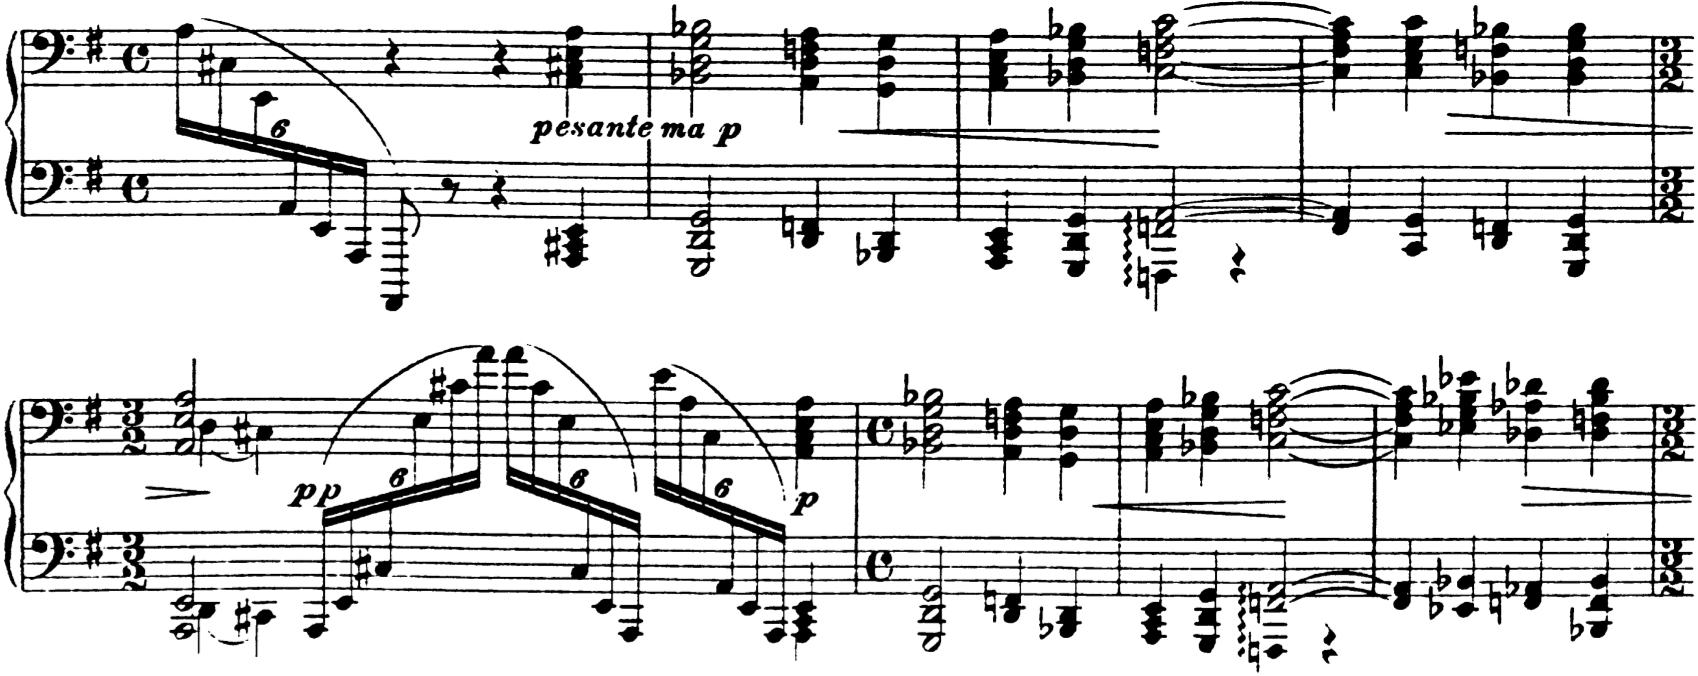
\includegraphics[width=12.5cm, keepaspectratio]{sonate-theme-E.png}
      &
      
\includegraphics[width=3cm, keepaspectratio]{op1-qr.png}
    \end{tabular}
  \end{bigcenter}
  \caption{\label{sonate-theme-1}Sonate en fa m Op.25, thème E.}
\end{figure}

\newpage

\subsubsection*{Le premier mouvement (?? mesures, $\sim$?m?s)}

\begin{figure}[!ht]
  \begin{bigcenter}
    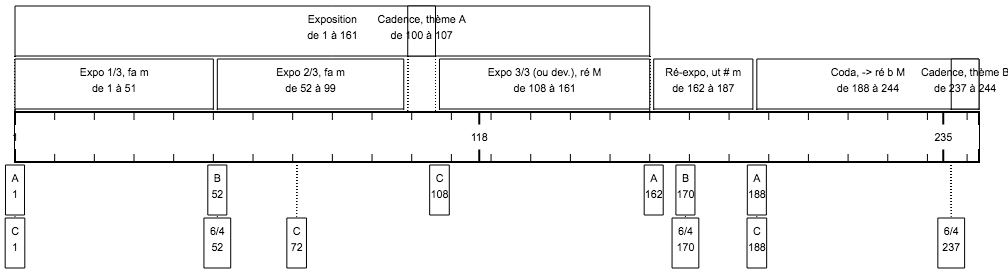
\includegraphics[width=15cm, keepaspectratio]{frise-mvt1.png}
  \end{bigcenter}
  \caption{\label{schema-3}Schéma du premier mouvement.}
\end{figure}

\subsubsection*{Le deuxième mouvement (?? mesures, $\sim$?m?s)}

Le deuxième mouvement à une forme tripartite A + B + A'.

\begin{figure}[!ht]
  \begin{bigcenter}
    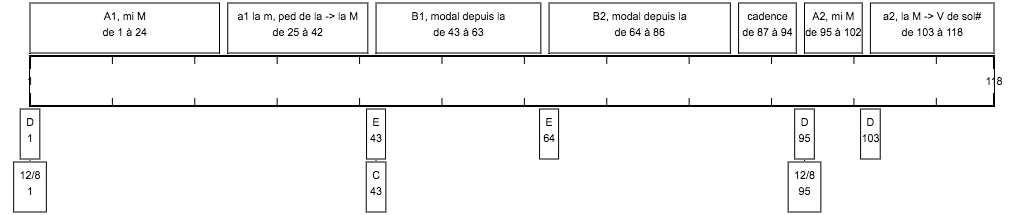
\includegraphics[width=15cm, keepaspectratio]{frise-mvt2.png}
  \end{bigcenter}
  \caption{\label{schema-3}Schéma du deuxième mouvement.}
\end{figure}

\subsubsection*{Le troisième mouvement (92 mesures, $\sim$2m8s)}

Dans les grandes sonates du XIX\ieme siècle, le troisième mouvement est très souvent un scherzo, c'est-à-dire une forme termaire, la plupart du temps à 3/4, héritée du menuet. Dans le cas de la sonate de Liapounov, nous avons trois variations en sol$\sharp$ mineur sur le thème B. Il ne s'agit pas réellement d'un scherzo mais la partition porte tout de même l'indication \emph{scherzando}. L'écriture \emph{Allegro vivo} à 6/8, au lieu de 6/4 dans le premier mouvement, confère un caractère qui avance et rythmé. Il s'agit du plus court mouvement de la sonate.

La forme est la suivante : intro évoquant le thème B (8 mesures, sol$\sharp$ mineur) + thème B (12 mesures, sol$\sharp$ mineur) + élément non thématique avec cadence (14 mesures, si majeur retour en sol$\sharp$ mineur) + variation ornementale du thème B (8 mesures, sol$\sharp$ mineur) + élément non thématique avec cadence (10 mesures, la majeur, retour en sol$\sharp$ mineur) + variation ornementale du thème B (8 mesures, sol$\sharp$ mineur) + élément non thématique avec cadence (12 mesures, do$\sharp$ majeur, retour vers sol$\sharp$ mineur) + codetta basée sur le thème B non varié (20 mesures, en sol$\sharp$ mineur modulant, se dirige vers fa mineur (= la tonalité principale de la sonate)).

\subsubsection*{Le quatrième mouvement (144 mesures, $\sim$7m10s)}

De même que dans le premier concerto de Liszt, qui est l'une des premières forme-sonates cycliques, nous allons voir que le dernier mouvement de la sonate de Liapounov fait office de ré-exposition (96 premières meseures) puis de coda (48 dernières mesures).

\paragraph{La ré-exposition}

Commençons par analyser la ré-exposition. Celle-ci commence sur un cinquième degré de fa avec le retour, pour la première fois depuis le premier mouvement, d'une version dégradée du thème A à la basse. Les 20 premières mesures ne sont qu'une préparation au retour du thème A en fa mineur meseure 21. C'est là que commance réellement la ré-exposition. Le thème A2 se fait entendre mesure 25 sur un cinquième degré. Puis Lyapounov fait à nouveau entendre A et A2 en la$\flat$ mineur. Mesure 37, la version majorisée du thème A se fait entendre en do$\flat$ majeur. Enfin nous, nous glissons, par modulations chromatiques succéssives, vers un cinquième degré de ré$\flat$ majeur mesures 45 et 46. Il s'agit de la fin de la première sous-partie de la ré-exposition.

À la mesure 47 (\emph{Meno mosso}), commence le thème C en ré$\flat$ majeur comme c'était déjà le cas dans le premier mouvement d'exposition puis à la tièrce en sol$\flat$ majeur. Les deux occurences du thème C sont sur pédale de ré$\flat$ (pédale de tonique). Puis, le thème A se fait à nouveau entrendre en ré$\flat$ majeur, puis à la seconde en mi$\flat$ mineur. Les deux occurences du thème A sont cette fois sur pédale de la$\flat$ (pédale de dominante).
Nous arrivons ensuite, mesure 63 sur le \emph{piano}, sur une grande pédale de dominante de fa qui demeurera jusqu'au \emph{Più animato} mesure 82. Elle fait entendre les thèmes C et une variante de B2. Il s'agit de la fin de la deuxième sous-partie de la ré-exposition.

Le \emph{Più animato} est de retour en fa mineur. Il fait entendre le thème B2 puis une cadence de dix mesures jusqu'à la double barre avant le 12/8. C'est la fin de la ré-exposition.

\begin{figure}[!ht]
  \begin{bigcenter}
    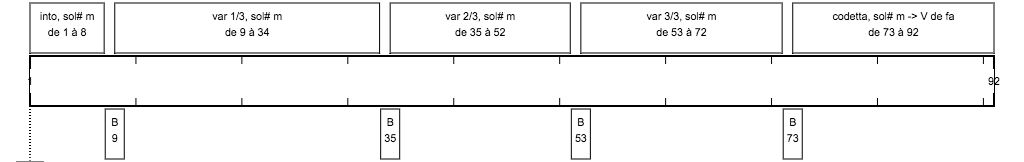
\includegraphics[width=15cm, keepaspectratio]{frise-mvt3.png}
  \end{bigcenter}
  \caption{\label{schema-3}Schéma du troisième mouvement.}
\end{figure}

\paragraph{La coda}

La coda commence au 12/8 et se termine à la fin de l'œuvre. Elle est entièrement écrite en fa majeur et se divise en deux parties. La première partie commence au \emph{Andante maestoso} et se termine juste avant l'\emph{L'istesso tempo} sur la demie-cadence de fa. Elle est construite à partir du thème D (en mi majeur dans le deuxième mouvement) et l'écriture pianistique évoque très clairement Mazeppa dans les \emph{études d'exécution transcendante} de Liszt (voir figure \ref{mazeppa}). La seconde et dernière partie de la coda est basée sur le thème E à partir de fa (à partir de la dans le deuxième mouvement). La sonate se termine par dix mesures de cadence parfaite en fa majeur, aussi paisiblement qu'à la fin de la sonate en si de Liszt.

\begin{figure}[!ht]
  \begin{bigcenter}
    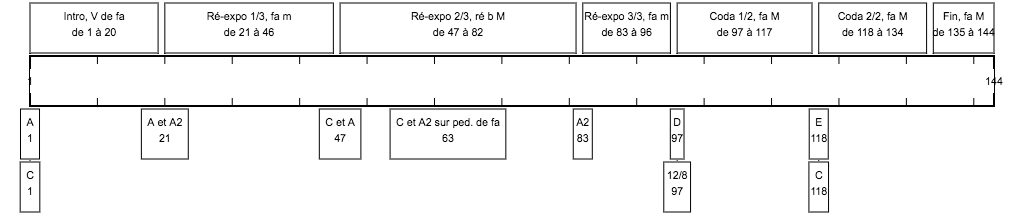
\includegraphics[width=15cm, keepaspectratio]{frise-mvt4.png}
  \end{bigcenter}
  \caption{\label{schema-4}Schéma du quatrième mouvement.}
\end{figure}

\begin{figure}[!p]
  \begin{bigcenter}
    \begin{tabular}{lr}
      \vspace*{0.0cm}
      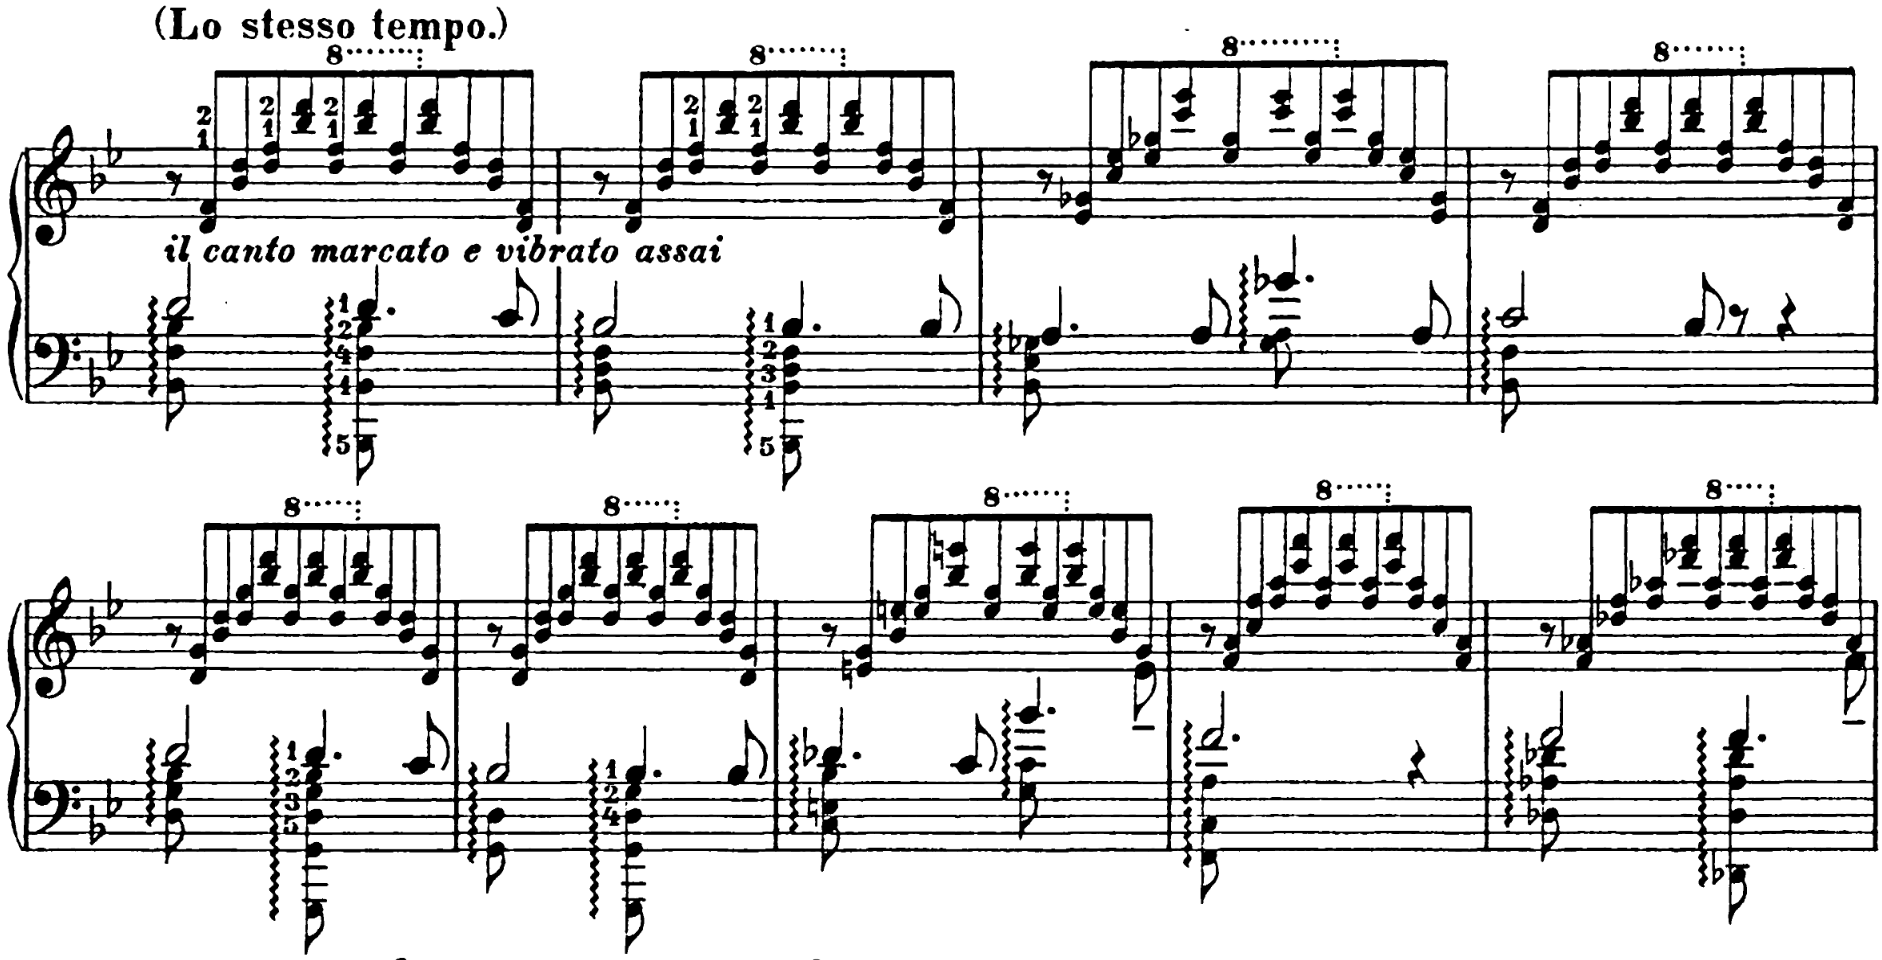
\includegraphics[width=12.5cm, keepaspectratio]{mazeppa.png}
      &
      
\includegraphics[width=3cm, keepaspectratio]{mazeppa-qr.png}
      \\
      \vspace{0.5cm} &
      \\
      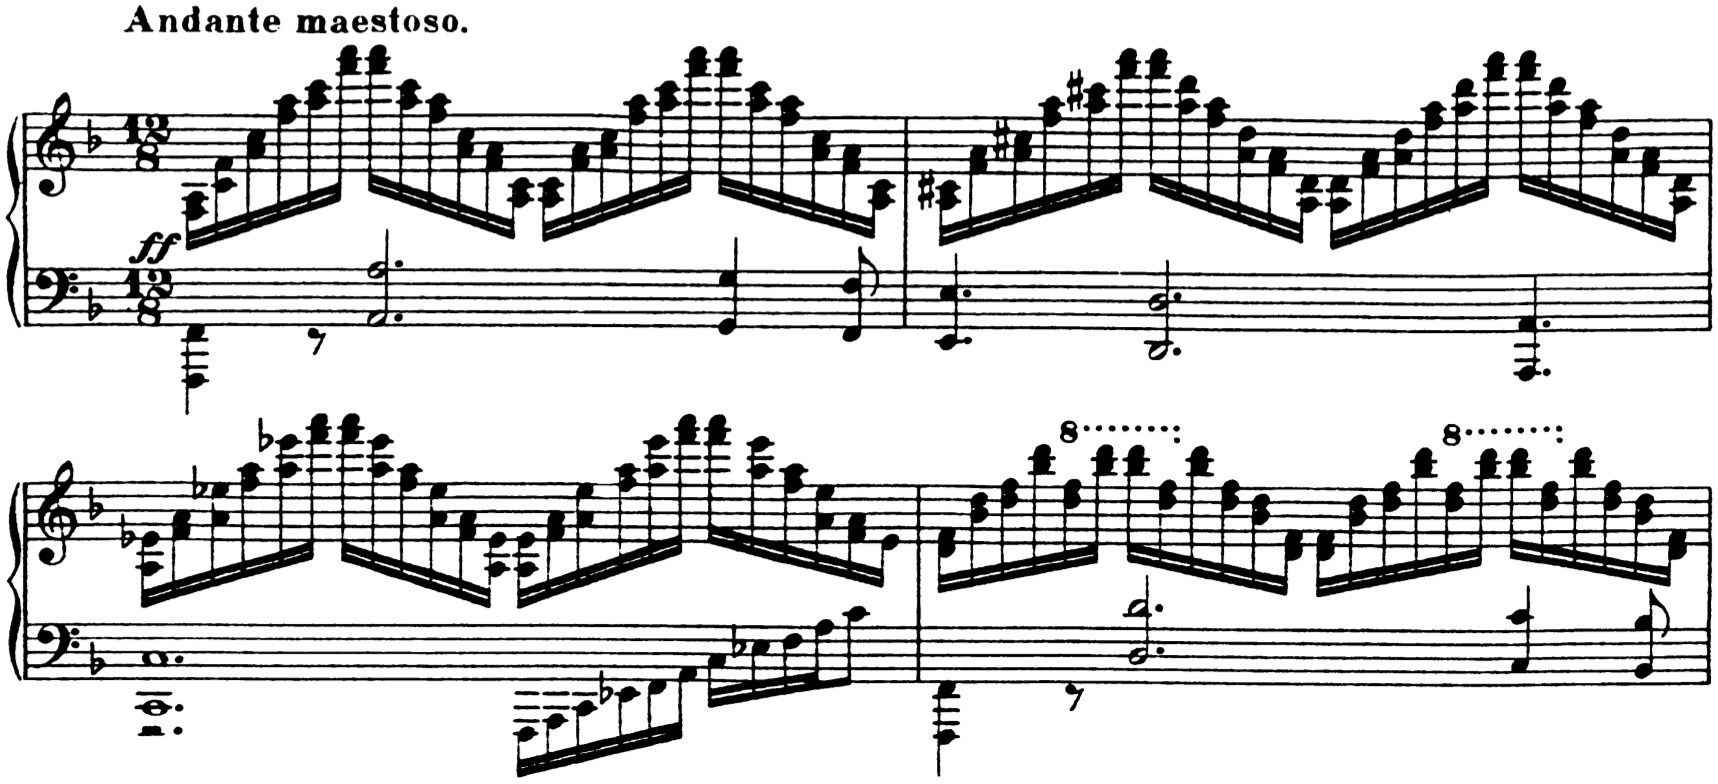
\includegraphics[width=12.5cm, keepaspectratio]{sonate-coda.png}
      &
      
\includegraphics[width=3cm, keepaspectratio]{sonate-qr.png}
    \end{tabular}
  \end{bigcenter}
  \caption{\label{mazeppa}Comparaison de \emph{Mazeppa} de Liszt (en haut) et du début de la coda de la sonate Op.27 de Liapounov (en bas).}
\end{figure}

%%%%%%%%%%%%%%%%%%%%%%%%%%%%%%%%%%%%%%%%%%%%%%%%%%%%%%%%%%%%%%%%%%%%%%%%%%%%%
